\documentclass[12pt, twoside]{article}
\input{../preamble}

\fancyhead[LE]{\thepage}
\fancyhead[RO]{\thepage}
\fancyhead[LO]{La Scuola d'Italia / Dr.\ Huson / IB Math: Kinematics --- Solutions \\* 11 March 2026}

\begin{document}
\subsubsection*{5.3 Classwork: Interpreting Motion Graphs --- Solutions}

\begin{enumerate}[itemsep=0.4cm]

%--- Problem 1: Displacement-time graph ---
\item The displacement $s$ (metres) of a particle from the origin is shown
      for $0 \leq t \leq 10$.

\begin{center}
\vspace{-0.3cm}
\begin{tikzpicture}[scale=0.5]
  \draw[-{Stealth}] (-0.5,0) -- (11,0) node[right] {$t$ (s)};
  \draw[-{Stealth}] (0,-4.5) -- (0,6.5) node[above] {$s$ (m)};
  \foreach \x in {1,...,10} \draw[gray!30] (\x,-4.5)--(\x,6.5);
  \foreach \y in {-4,...,6} \draw[gray!30] (-0.5,\y)--(11,\y);
  \foreach \x in {2,4,6,8,10} \draw (\x,0.1)--(\x,-0.1) node[below]{\small\x};
  \foreach \y in {-4,-2,2,4,6} \draw (0.1,\y)--(-0.1,\y) node[left]{\small\y};
  \node[below left] at (0,0) {\small 0};
  \draw[very thick]
    (0,2) -- (3,6) -- (6,6) -- (8,-2) -- (10,-4);
  \foreach \pt in {(0,2),(3,6),(6,6),(8,-2),(10,-4)}
    \fill \pt circle (3pt);
\end{tikzpicture}
\vspace{-0.3cm}
\end{center}

\begin{enumerate}[itemsep=0.1cm]
  \item Write down the initial displacement of the particle. \hfill [1]
  \item Find the velocity during $0 \leq t \leq 3$. \hfill [2]
  \item Describe the motion of the particle during $3 \leq t \leq 6$. \hfill [1]
  \item Find the velocity during $6 \leq t \leq 8$. \hfill [2]
  \item At what time does the particle pass through the origin? \hfill [2]
  \item Find the total \textbf{distance} travelled from $t = 0$ to $t = 10$. \hfill [3]
  \item Find the \textbf{displacement} from $t = 0$ to $t = 10$. \hfill [1]
\end{enumerate}

\vfill

\begin{tikzpicture}
  \draw (0,0) rectangle (15.5,11);
  \node[anchor=north west, inner sep=0.40cm] at (0,11) {%
    \begin{minipage}[t]{14.7cm}%
      \textbf{Solutions}\\[0.4cm]
      \textbf{(a)}\enspace $s(0) = \mathbf{2}$ m\\[0.4cm]
      \textbf{(b)}\enspace $v = \dfrac{6 - 2}{3 - 0} = \dfrac{4}{3} \approx \mathbf{1.33}$
        m\,s$^{-1}$\\[0.4cm]
      \textbf{(c)}\enspace The particle is stationary (displacement is constant at 6\,m).\\[0.4cm]
      \textbf{(d)}\enspace $v = \dfrac{-2 - 6}{8 - 6} = \dfrac{-8}{2}
        = \mathbf{-4}$ m\,s$^{-1}$\\[0.4cm]
      \textbf{(e)}\enspace The line from $(6, 6)$ to $(8, -2)$ has equation
        $s = 6 - 4(t - 6)$.\\[0.1cm]
      \hspace*{2.5em}Set $s = 0$: \enspace $6 - 4(t - 6) = 0
        \;\Rightarrow\; t - 6 = \dfrac{6}{4} = 1.5
        \;\Rightarrow\; t = \mathbf{7.5}$ s\\[0.4cm]
      \textbf{(f)}\enspace Distance $= |6 - 2| + |6 - 6| + |-2 - 6| + |-4 - (-2)|
        = 4 + 0 + 8 + 2 = \mathbf{14}$ m\\[0.4cm]
      \textbf{(g)}\enspace Displacement $= s(10) - s(0) = -4 - 2 = \mathbf{-6}$ m%
    \end{minipage}%
  };
\end{tikzpicture}

\newpage

%--- Problem 2: Matching graphs ---
\item The graphs below show the displacement and velocity of a particle.
      Match each description (i)--(iv) to the correct time interval. \hfill [4]

\begin{center}
\begin{tikzpicture}[scale=0.5]
  \draw[-{Stealth}] (-0.5,0) -- (9,0) node[right] {$t$};
  \draw[-{Stealth}] (0,-1.5) -- (0,5.5) node[left] {$s$};
  \foreach \x in {2,4,6,8} \draw (\x,0.1)--(\x,-0.1) node[below]{\small\x};
  \draw[very thick]
    (0,0) -- (2,4) -- (4,4) -- (6,2) -- (8,2);
  \foreach \pt in {(0,0),(2,4),(4,4),(6,2),(8,2)}
    \fill \pt circle (3pt);
  \node[above] at (4.5,5.5) {\textbf{Displacement--time graph}};
\end{tikzpicture}
\hspace{1.5cm}
\begin{tikzpicture}[scale=0.5]
  \draw[-{Stealth}] (-0.5,0) -- (9,0) node[right] {$t$};
  \draw[-{Stealth}] (0,-2.5) -- (0,4.5) node[above] {$v$};
  \foreach \x in {2,4,6,8} \draw (\x,0.1)--(\x,-0.1) node[below]{\small\x};
  \draw[very thick]
    (0,2) -- (2,2) -- (2,0) -- (4,0) -- (4,-1) -- (6,-1) -- (6,0) -- (8,0);
  \node[above] at (4.5,4.5) {\textbf{Velocity--time graph}};
\end{tikzpicture}
\end{center}

\begin{enumerate}[label=(\roman*), itemsep=0.1cm]
  \item The particle is moving forward at constant speed.
  \item The particle is stationary.
  \item The particle is moving backward at constant speed.
  \item The particle is stationary (for the second time).
\end{enumerate}

\vfill

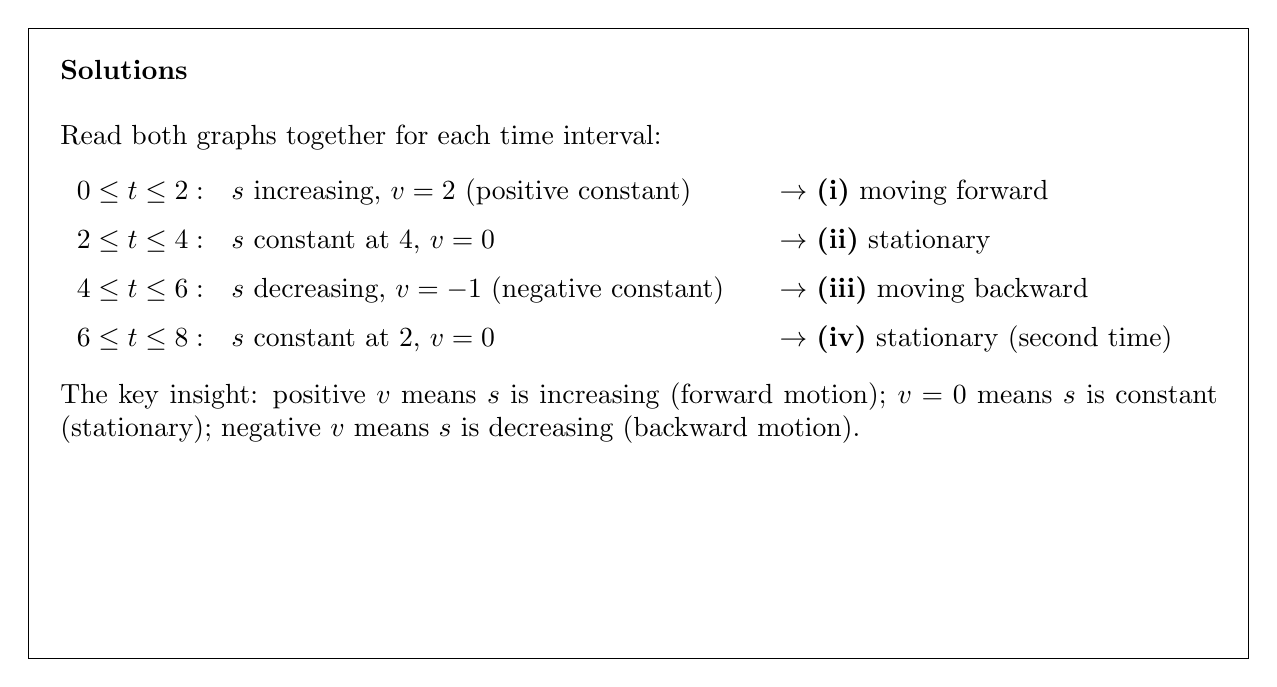
\begin{tikzpicture}
  \draw (0,0) rectangle (15.5,8);
  \node[anchor=north west, inner sep=0.40cm] at (0,8) {%
    \begin{minipage}[t]{14.7cm}%
      \textbf{Solutions}\\[0.4cm]
      Read both graphs together for each time interval:\\[0.3cm]
      \begin{tabular}{r@{\;:\quad}l@{\qquad}l}
        $0 \leq t \leq 2$ & $s$ increasing, $v = 2$ (positive constant)
          & $\rightarrow$ \textbf{(i)} moving forward \\[0.2cm]
        $2 \leq t \leq 4$ & $s$ constant at 4, $v = 0$
          & $\rightarrow$ \textbf{(ii)} stationary \\[0.2cm]
        $4 \leq t \leq 6$ & $s$ decreasing, $v = -1$ (negative constant)
          & $\rightarrow$ \textbf{(iii)} moving backward \\[0.2cm]
        $6 \leq t \leq 8$ & $s$ constant at 2, $v = 0$
          & $\rightarrow$ \textbf{(iv)} stationary (second time)
      \end{tabular}\\[0.3cm]
      The key insight: positive $v$ means $s$ is increasing (forward motion);
      $v = 0$ means $s$ is constant (stationary); negative $v$ means $s$ is
      decreasing (backward motion).%
    \end{minipage}%
  };
\end{tikzpicture}

\newpage

%--- Problem 3: Velocity-time graph ---
\item The velocity $v$ (m\,s$^{-1}$) of a cyclist is shown for $0 \leq t \leq 12$ seconds.

\begin{center}
\vspace{-0.3cm}
\begin{tikzpicture}[scale=0.55]
  \draw[-{Stealth}] (-0.5,0) -- (13,0) node[right] {$t$ (s)};
  \draw[-{Stealth}] (0,-3.5) -- (0,7.5) node[above] {$v$ (m\,s$^{-1}$)};
  \foreach \x in {1,...,12} \draw[gray!30] (\x,-3.5)--(\x,7.5);
  \foreach \y in {-3,...,7} \draw[gray!30] (-0.5,\y)--(13,\y);
  \foreach \x in {2,4,6,8,10,12} \draw (\x,0.1)--(\x,-0.1) node[below]{\small\x};
  \foreach \y in {-2,2,4,6} \draw (0.1,\y)--(-0.1,\y) node[left]{\small\y};
  \node[below left] at (0,0) {\small 0};
  \draw[very thick]
    (0,0) -- (4,6) -- (8,6) -- (10,0) -- (12,-2);
  \foreach \pt in {(0,0),(4,6),(8,6),(10,0),(12,-2)}
    \fill \pt circle (3pt);
\end{tikzpicture}
\vspace{-0.3cm}
\end{center}

\begin{enumerate}[itemsep=0.1cm]
  \item Find the acceleration during $0 \leq t \leq 4$. \hfill [2]
  \item Describe the motion during $4 \leq t \leq 8$. \hfill [1]
  \item Find the acceleration during $8 \leq t \leq 10$. \hfill [2]
  \item Find the total distance travelled from $t = 0$ to $t = 10$. \hfill [3]
  \item What does the negative velocity during $10 < t \leq 12$ tell you? \hfill [1]
  \item Find the total distance travelled from $t = 0$ to $t = 12$. \hfill [2]
  \item Find the average speed of the cyclist over the 12-second interval. \hfill [2]
\end{enumerate}

\vfill

\begin{tikzpicture}
  \draw (0,0) rectangle (15.5,10);
  \node[anchor=north west, inner sep=0.40cm] at (0,10) {%
    \begin{minipage}[t]{14.7cm}%
      \textbf{Solutions} \emph{Distance = area under the velocity--time graph.}\\[0.4cm]
      \textbf{(a)}\enspace $a = \dfrac{6 - 0}{4 - 0} = \dfrac{6}{4}
        = \mathbf{1.5}$ m\,s$^{-2}$\\[0.4cm]
      \textbf{(b)}\enspace Constant velocity of 6\,m\,s$^{-1}$
        (zero acceleration, moving forward at constant speed).\\[0.4cm]
      \textbf{(c)}\enspace $a = \dfrac{0 - 6}{10 - 8} = \dfrac{-6}{2}
        = \mathbf{-3}$ m\,s$^{-2}$\\[0.4cm]
      \textbf{(d)}\enspace Triangle ($0$ to $4$): $\frac{1}{2} \times 4 \times 6 = 12$ m\\[0.1cm]
      \hspace*{2.5em}Rectangle ($4$ to $8$): $4 \times 6 = 24$ m\\[0.1cm]
      \hspace*{2.5em}Triangle ($8$ to $10$): $\frac{1}{2} \times 2 \times 6 = 6$ m\\[0.1cm]
      \hspace*{2.5em}Total $= 12 + 24 + 6 = \mathbf{42}$ m\\[0.4cm]
      \textbf{(e)}\enspace The cyclist is moving in the opposite (negative) direction.\\[0.4cm]
      \textbf{(f)}\enspace Triangle ($10$ to $12$, below axis):
        $\frac{1}{2} \times 2 \times 2 = 2$ m.
        \enspace Total $= 42 + 2 = \mathbf{44}$ m\\[0.4cm]
      \textbf{(g)}\enspace Average speed
        $= \dfrac{44}{12} = \dfrac{11}{3} \approx \mathbf{3.67}$
        m\,s$^{-1}$%
    \end{minipage}%
  };
\end{tikzpicture}

\end{enumerate}
\end{document}
